\documentclass[style=unh]{powerdot}
\usepackage{graphicx}

\pdsetup{
  lf={Ethan Burns (UNH)},
  rf = {Parallel Best-First Heuristic Search},
  list={itemsep=8pt}}


\title{Parallel Best-First Heuristic Search}
\author{Ethan Burns \vspace{0.2in} \\
  
\includegraphics[height=0.4in]{figures/unh-logo-words.eps} \\
  Department of Computer Science \\
  {\tt eaburns} at {\tt unh.edu}}
\date{\mbox{}}

\begin{document}
\maketitle

% ------------------------------------------------------------

\section[slide=false]{Introduction}

% --------------------

\begin{slide}{Goal}
  \vspace{1in}
  \begin{center}
    Solve small problems as fast as possible \\
    {\tiny Using multi-core}
  \end{center}

\end{slide}

% --------------------

\begin{slide}{Motivation}
  \onslide{1,2}{
    \begin{center}
      Why multi-core?
    \end{center}

    \begin{itemize}
    \item Parallelism is replacing horse power for speed
    \end{itemize}
  }
  \vspace{.3in}
  \onslide*{2}{
    \begin{center}
      Why small problems?
    \end{center}

    \begin{itemize}
    \item Trend in research is to solve larger and larger problems
    \item Large problems are hard to solve
    \item Re-learn to solve small problems using parallelism for speed
    \item Real-time
    \end{itemize}
  }
\end{slide}

% ------------------------------------------------------------

\section{Background}

% --------------------

%% \begin{slide}{PRA*}
%%   \vspace{.2in}
%%   \begin{center}
%%     Parallel Retracting A*
%%   \end{center}

%%   \vspace{.1in}

%%   \begin{itemize}[type=1]
%%   \item Each processor is a hash bucket
%%   \item Each search node hashes to a single processor
%%   \item Processors expand their nodes and pass children to
%%     appropriate buckets
%%   \item Uses a retracting scheme for memory efficiency
%%   \end{itemize}
%% \end{slide}

% --------------------

\begin{slide}{SDD}
  \vspace{.2in}
  \begin{center}
    Structured Duplicate Detection
  \end{center}

  \onslide*{1}{
    \begin{itemize}
    \item External memory graph search
    \item Decompose search graph by \emph{projecting} nodes into an abstract space
    \item \emph{Duplicate detection scopes}
    \end{itemize}
  }
  \onslide*{2}{
    \begin{center}
      \includegraphics[width=2in]{figures/disjoint-scopes1} \\
      15-Puzzle projected on the blank
    \end{center}
  }
  \onslide*{3}{
    \begin{itemize}
    \item NBlock: all of the search nodes in the same abstract state
    \item Breadth-first heuristic search
    \item Single $depth$ layer at a time
    \end{itemize}
  }
\end{slide}

% --------------------

\begin{slide}{PSDD}
  \vspace{.2in}
  \begin{center}
    Parallel Structured Duplicate Detection
  \end{center}
  \onslide*{1}{
    \begin{itemize}
    \item Multiple processors search \emph{disjoint duplicate detection
      scopes} concurrently.
    \item Search proceeds in a breadth-first manor, as in SDD
    \item Processors synchronize before switching layers
    \end{itemize}
  }
  \onslide*{2}{
    \begin{center}
      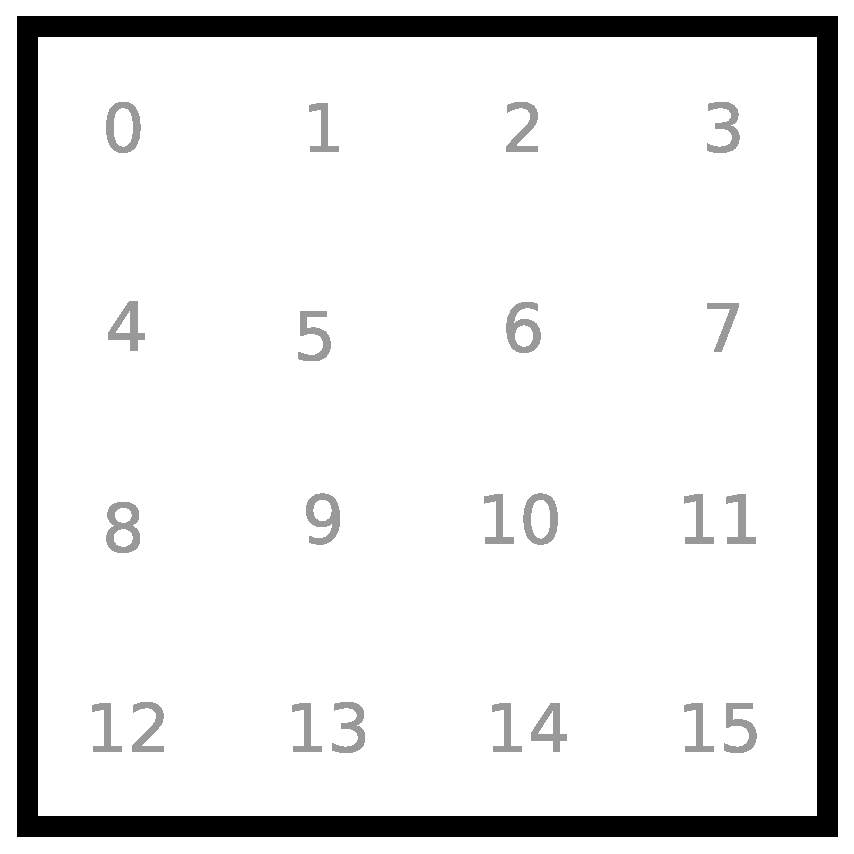
\includegraphics[width=2in]{figures/disjoint-scopes0} \\
    \end{center}
  }
  \onslide*{3}{
    \begin{center}
      \includegraphics[width=2in]{figures/disjoint-scopes1} \\
    \end{center}
  }
  \onslide*{4}{
    \begin{center}
      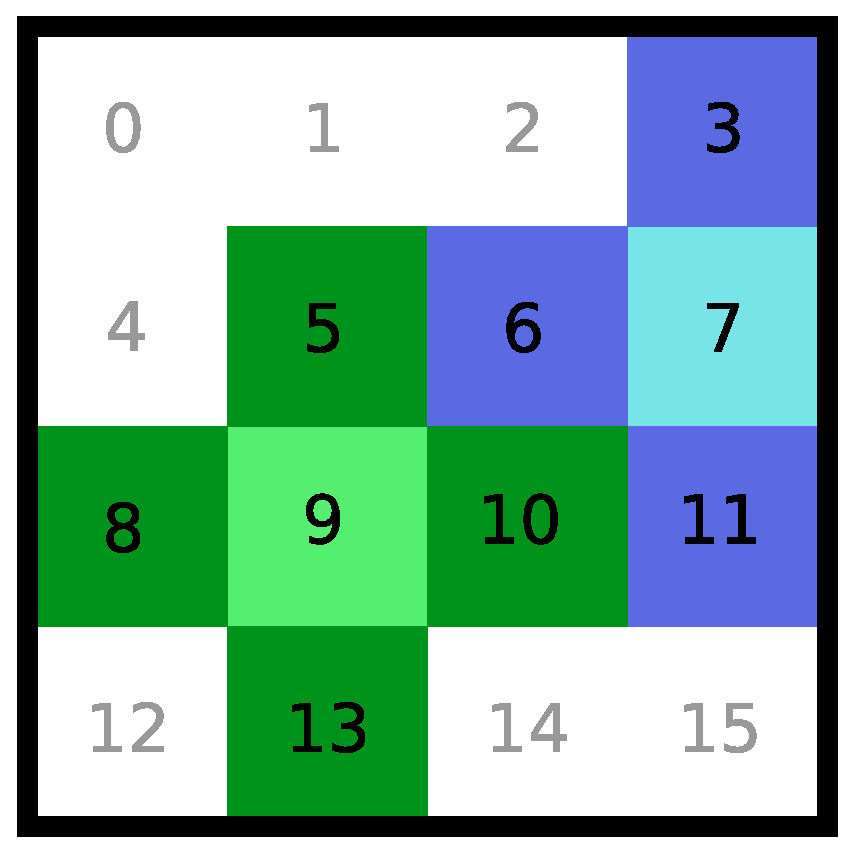
\includegraphics[width=2in]{figures/disjoint-scopes2} \\
    \end{center}
  }
  \onslide*{5}{
    \begin{center}
      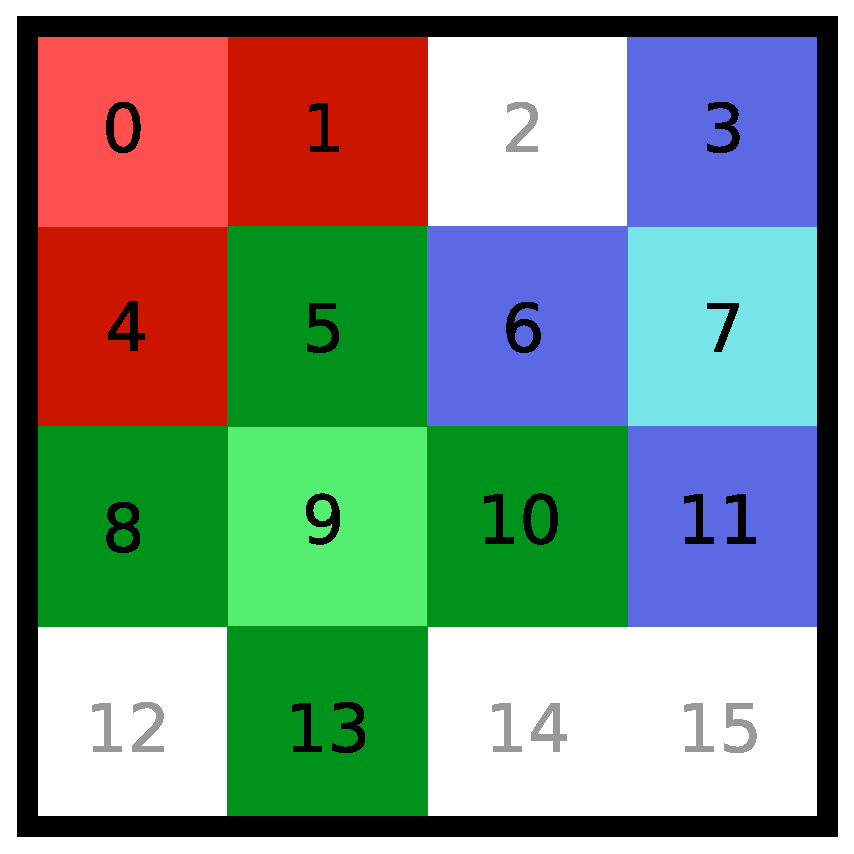
\includegraphics[width=2in]{figures/disjoint-scopes3} \\
    \end{center}
  }
  \onslide*{6}{
    \begin{center}
      \includegraphics[width=2in]{figures/disjoint-scopes4} \\
    \end{center}
  }
  \onslide*{7}{
    \begin{center}
      \includegraphics[width=2in]{figures/disjoint-scopes5} \\
    \end{center}
  }
  \onslide*{8}{
    \begin{center}
      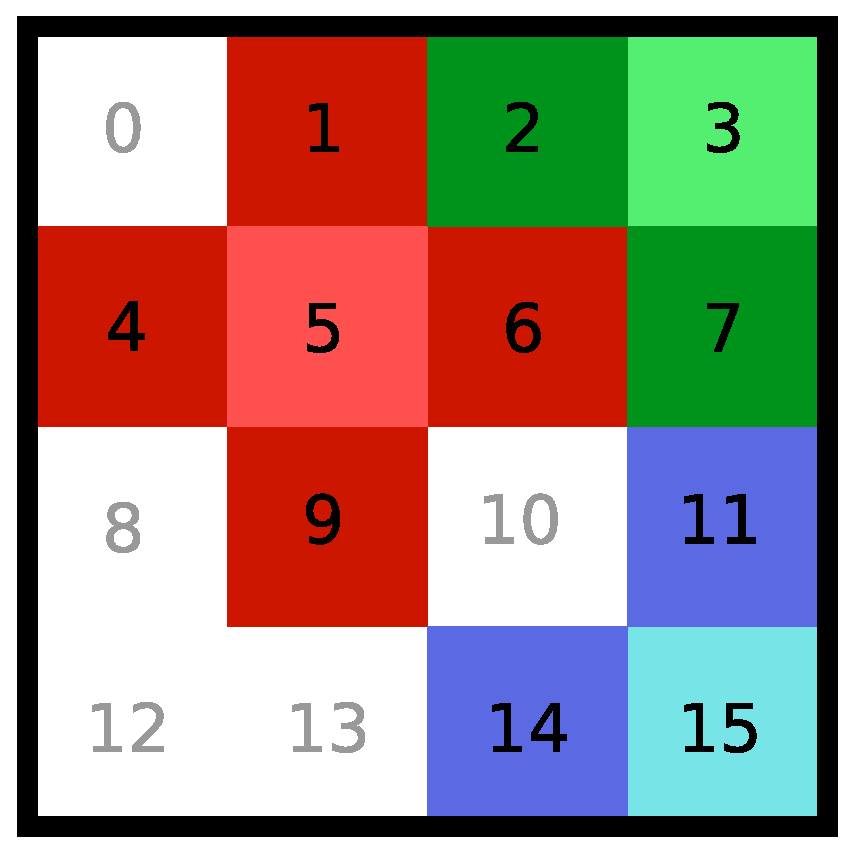
\includegraphics[width=2in]{figures/disjoint-scopes6} \\
    \end{center}
  }

  \onslide*{2,3,4,5,6,7,8} {
    \vspace{-.3in}
    \begin{center}
      15-Puzzle projected on the blank
    \end{center}
  }

\end{slide}

\begin{slide}{PSDD Variants}
  \vspace{.2in}
  \begin{center}
    Parallel Structured Duplicate Detection Variants
  \end{center}

  \begin{description}

  \item[Standard PSDD]
    Uses breadth-first heuristic search
  \item[Dynamic PSDD]
    Not really technically a variant -- Dynamic PSDD uses an initial
    weighted A* to get a cost bound, then performs standard PSDD.
  \item[Best-first PSDD]
    Uses $f$ value layers instead of $depth$ layers.
  \end{description}

\end{slide}

% --------------------

\begin{slide}{lA*}
  \vspace{.2in}
  \begin{center}
    Localized A*
  \end{center}

  \begin{itemize}
  \item Efficient memory search
  \item Prefer memory locality to strict best-firstyness
  \item \emph{Heap-of-heaps} $H = \langle H_0, H_1, ..., H_n \rangle$
  \item Heaps $H_i$ contain nodes in the same memory page
  \item Best heap, $H_0$, expanded while
    \begin{eqnarray*}
      (\mathop{\rm min}_{n \in H_0} f(n)) < (\mathop{\rm min}_{m \in H_1} f(m)) + \Delta
    \end{eqnarray*}
    where $H_1$ is the next best heap on $H$
  \end{itemize}

\end{slide}

% ------------------------------------------------------------

\section{PBNF}

% --------------------

\begin{slide}{PBNF}
  \vspace{.2in}
  \begin{center}
    Parallel Best NBlock First
  \end{center}

  \begin{itemize}
  \item Heap of free nblocks $H = \langle N_0, N_1, ..., N_n \rangle$
  \item Processors acquire the best disjoint nblocks
  \item NBlock, $N_0$, expanded while
    \begin{eqnarray*}
      (\mathop{\rm min}_{n \in N_0} f(n)) < (\mathop{\rm min}_{m \in N_{next}} f(m))
    \end{eqnarray*}
    where $N_{next}$ is the next best nblock on $H$
  \item Cleanup phase for optimal solutions
  \item Minimum expansions, $m$ to reduce contention
  \item No layer based synchronization
  \end{itemize}

\end{slide}

% --------------------

\begin{slide}{Safe PBNF}
  \vspace{.2in}
  \begin{center}
    Safe Parallel Best NBlock First
  \end{center}
  \onslide*{1}{
    \begin{center}
      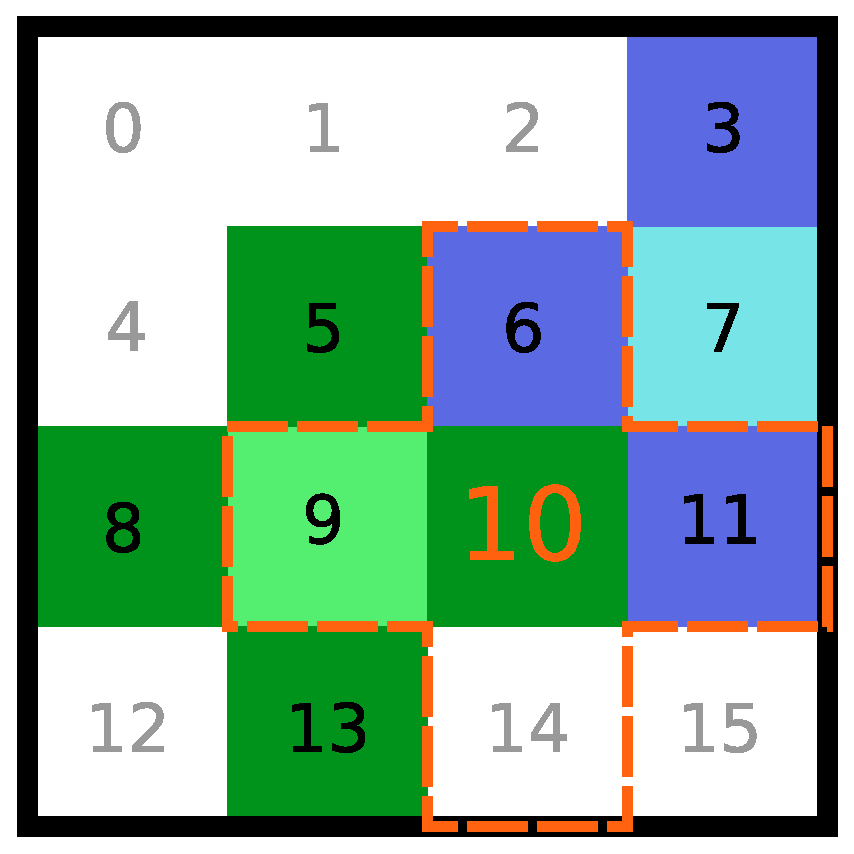
\includegraphics[width=2in]{figures/livelock0} \\
    \end{center}
  }
  \onslide*{2}{
    \begin{center}
      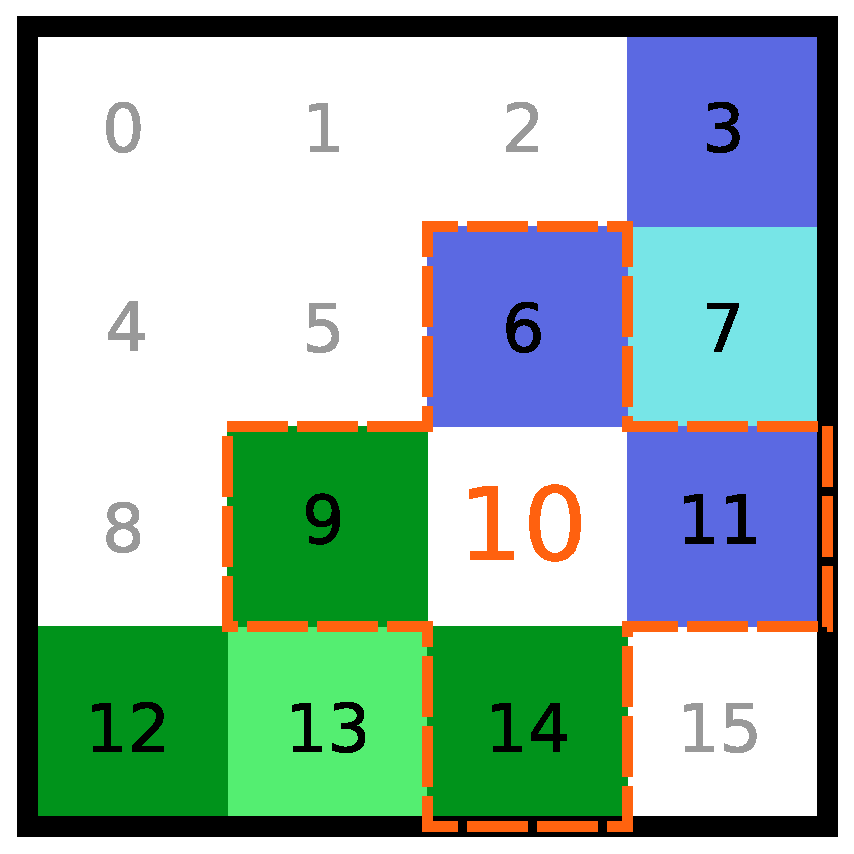
\includegraphics[width=2in]{figures/livelock1} \\
    \end{center}
  }
  \onslide*{3}{
    \begin{center}
      \includegraphics[width=2in]{figures/livelock2} \\
    \end{center}
  }
  \onslide*{4}{
    \begin{center}
      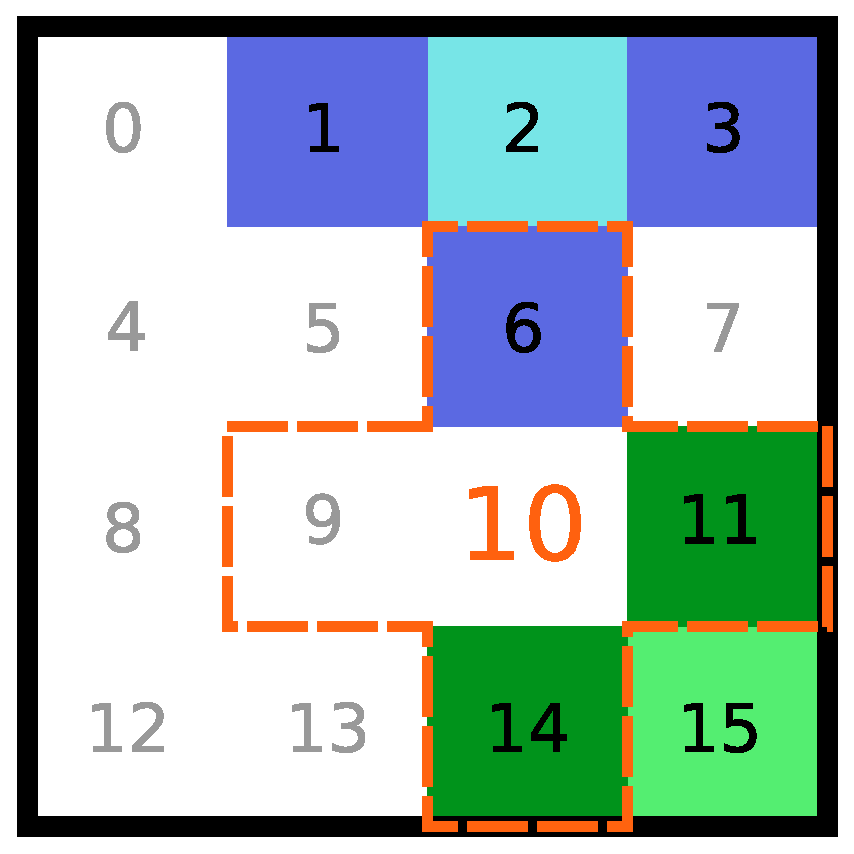
\includegraphics[width=2in]{figures/livelock3} \\
    \end{center}
  }
  \onslide*{5}{
    \begin{center}
      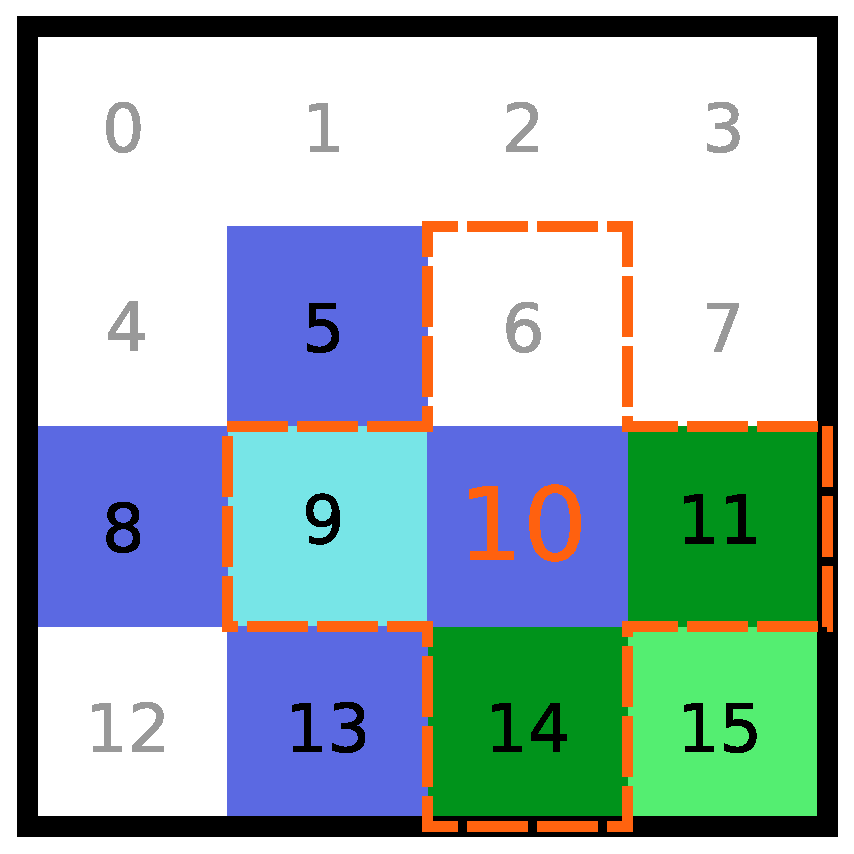
\includegraphics[width=2in]{figures/livelock4} \\
    \end{center}
  }
  \onslide*{6}{
    \begin{center}
      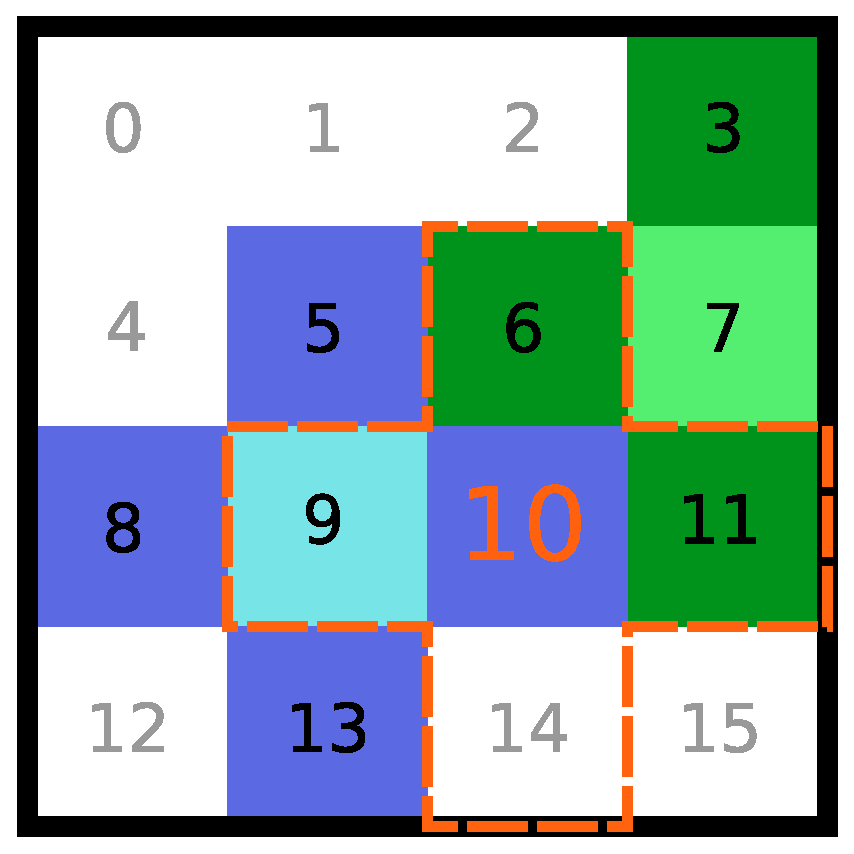
\includegraphics[width=2in]{figures/livelock5} \\
    \end{center}
  }
  \onslide*{7}{
    \begin{center}
      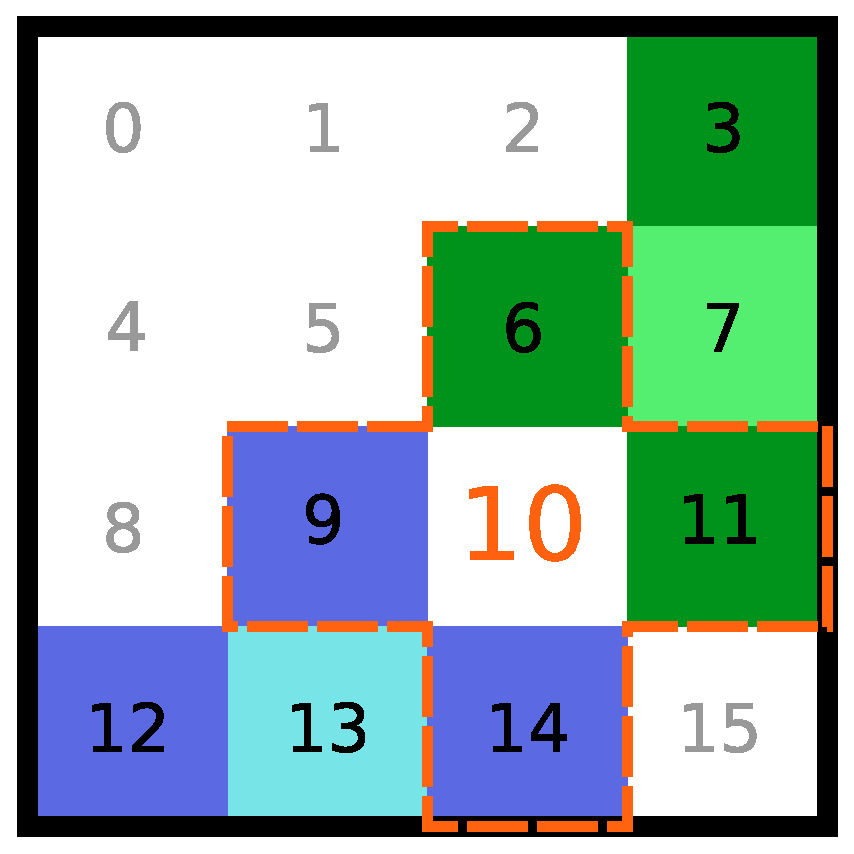
\includegraphics[width=2in]{figures/livelock6} \\
    \end{center}
  }
  \onslide*{8}{
    \begin{center}
      \includegraphics[width=2in]{figures/livelock7} \\
    \end{center}
  }
  \onslide*{9}{
    \begin{center}
      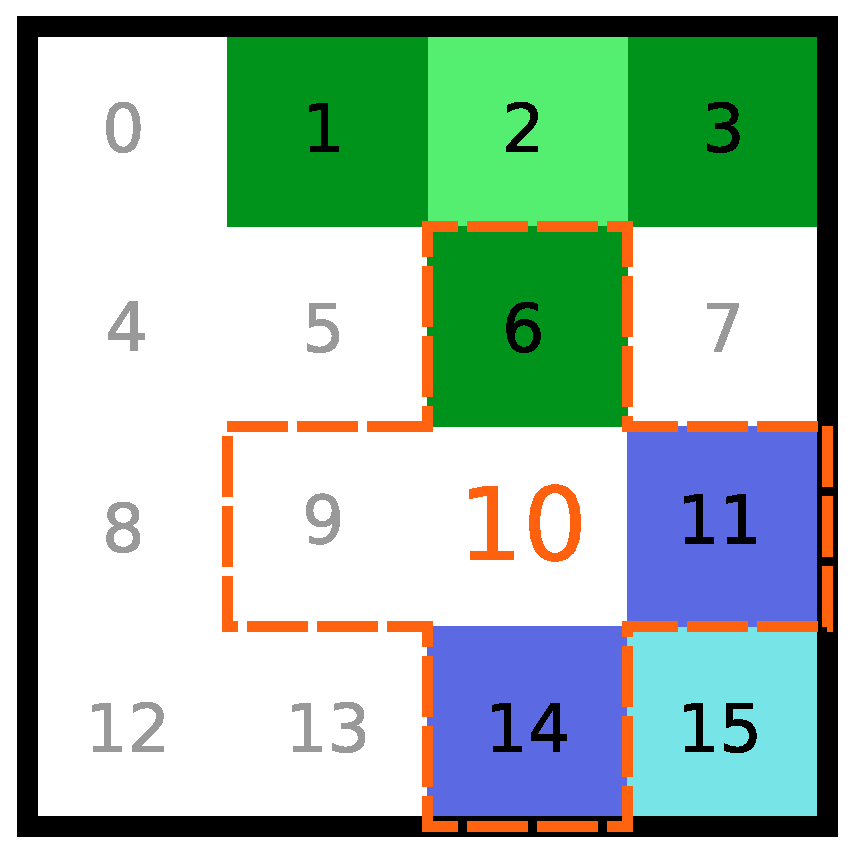
\includegraphics[width=2in]{figures/livelock8} \\
    \end{center}
  }
  \onslide*{10}{
    \begin{center}
      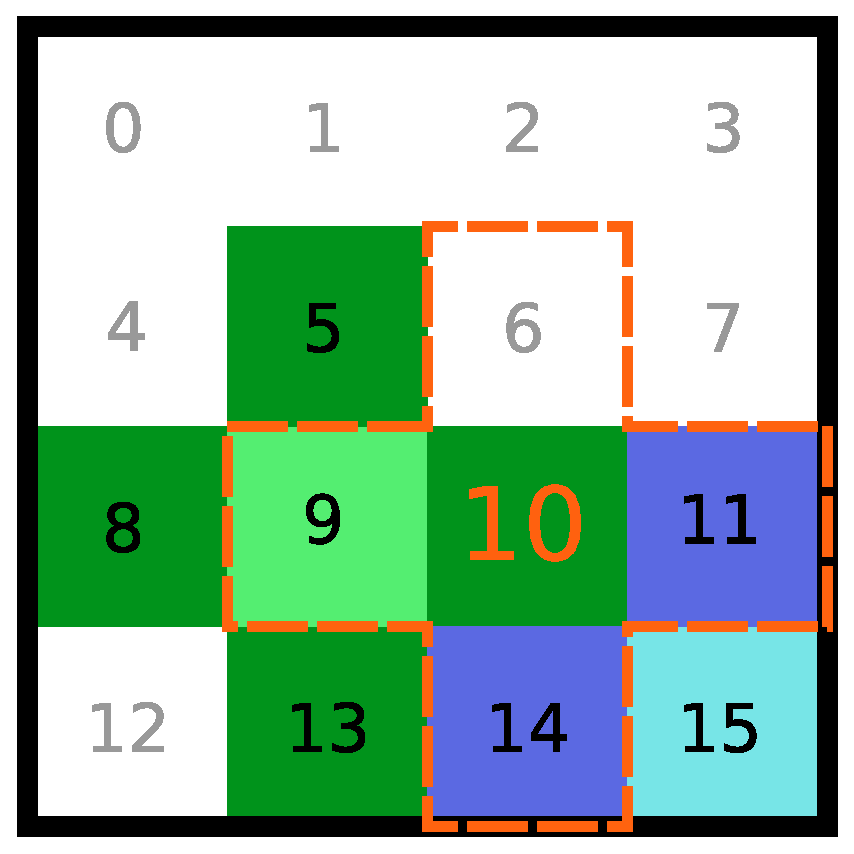
\includegraphics[width=2in]{figures/livelock9} \\
    \end{center}
  }
  \onslide*{11}{
    \begin{center}
      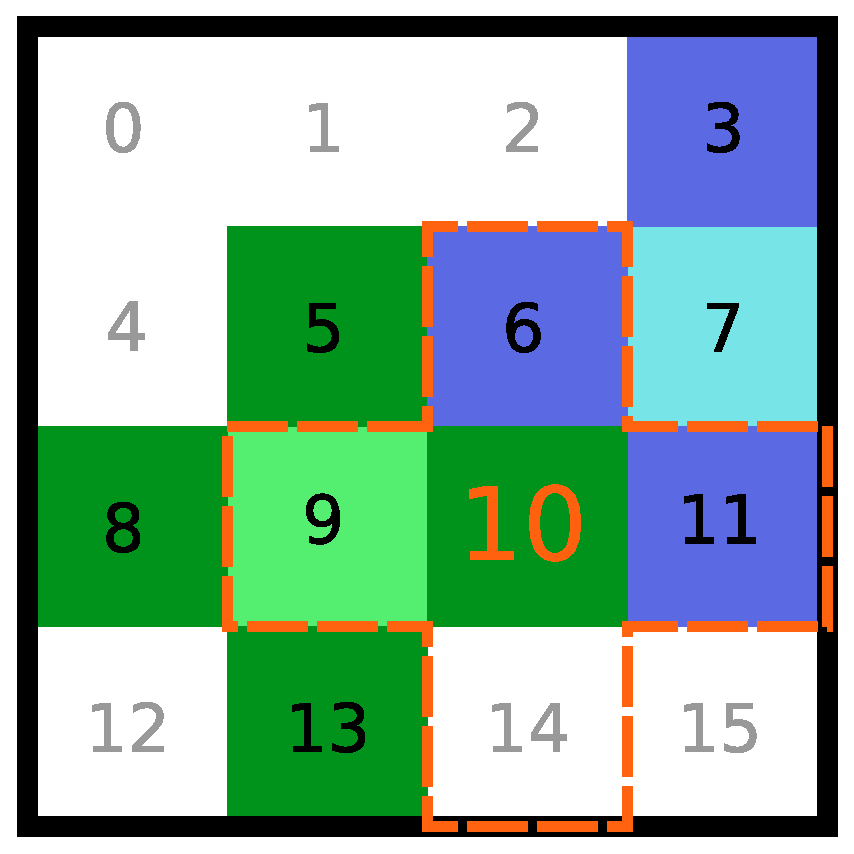
\includegraphics[width=2in]{figures/livelock0} \\
    \end{center}
  }

  \onslide*{1,2,3,4,5,6,7,8,9,10,11} {
    \vspace{-.3in}
    \begin{center}
      15-Puzzle projected on the blank
    \end{center}
  }

  \onslide*{12}{
    \begin{itemize}
    \item Mark nblocks as \emph{hot}
    \item Release nblocks which are interfering with hot nblocks
    \item Do not acquire scopes which interfere with hot nblocks
    \item $setcold()$ if not releasing
    \item Hot blocks must not interfere
    \item TLA+ model
    \end{itemize}
  }
  \onslide*{13}{
    \begin{center}
      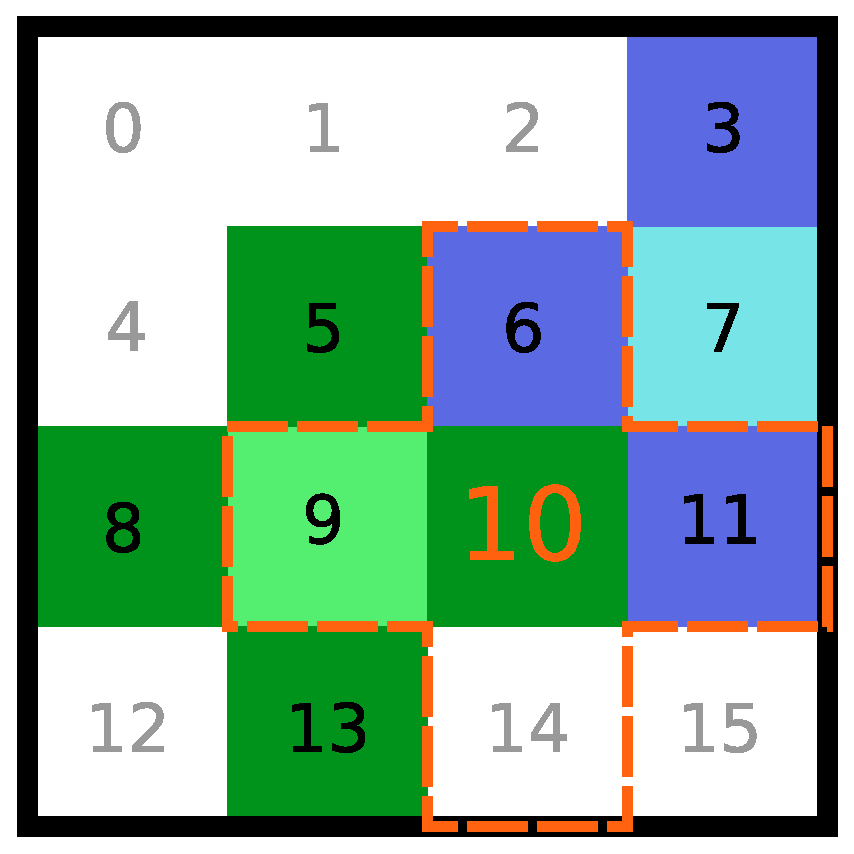
\includegraphics[width=2in]{figures/livelock0} \\
    \end{center}
  }
  \onslide*{14}{
    \begin{center}
      \includegraphics[width=2in]{figures/livelock1h} \\
    \end{center}
  }
  \onslide*{15}{
    \begin{center}
      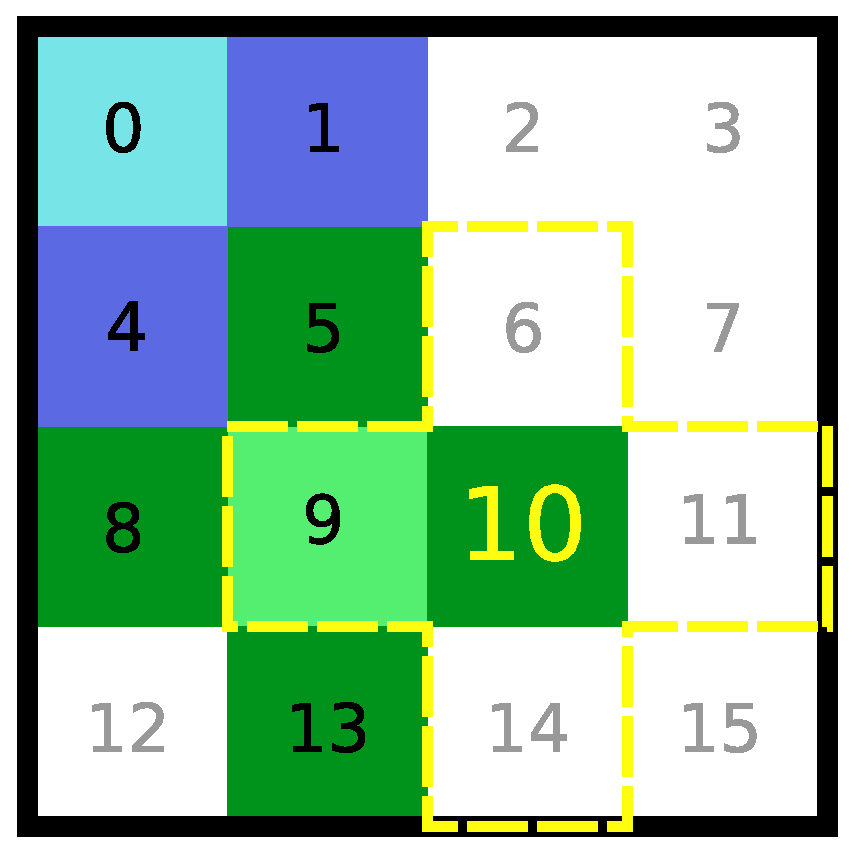
\includegraphics[width=2in]{figures/livelock2h} \\
    \end{center}
  }
  \onslide*{16}{
    \begin{center}
      \includegraphics[width=2in]{figures/livelock3h} \\
    \end{center}
  }
  \onslide*{17}{
    \begin{center}
      \includegraphics[width=2in]{figures/livelock4h} \\
    \end{center}
  }
  \onslide*{13,14,15,16,17} {
    \vspace{-.3in}
    \begin{center}
      15-Puzzle projected on the blank
    \end{center}
  }

\end{slide}

% --------------------

\begin{slide}{PBNF Variants}
  \vspace{.2in}
  \begin{center}
    Parallel Best NBlock First Variants
  \end{center}
  \begin{description}
  \item[PBNF] The standard PBNF algorithm
  \item[Safe PBNF] The safe PBNF algorithm
  \item[Weighted PBNF] PBNF with a weighted heuristic (no proving
    optimality phase).
  \item[Pessimistic PBNF] PBNF with a pessimistic heuristic (no proving
    optimality phase).
  \item[Optimistic PBNF] Weighted PBNF as the greedy phase of an optimistic search.
  \item[Possibly many more...]
  \end{description}
\end{slide}

% ------------------------------------------------------------

\section{Experiments}

% --------------------

\begin{slide}{Parameters}
  \begin{center}
    What are they?
  \end{center}
  \begin{itemize}
    \item $\frac{nblocks}{thread}$ -- applicable in grid world
    \item $min-expansions$ -- applicable for PBNF
  \end{itemize}

  \pause
  \vspace{.4in}

  \begin{center}
    How were they chosen?
  \end{center}
  \begin{itemize}
    \item Experimentation
  \end{itemize}
\end{slide}

% --------------------

\begin{slide}{Grid World}
  \onslide*{1}{
    \begin{description}
    \item [Width] 2000
    \item [Height] 1200
    \item [Obstacle distribution] Uniform 0.25
    \item [Costs] Unit and Life
    \item [Start] Bottom Left
    \item [Goal] Bottom Right
    \item[Projection] $(row {\rm MOD} M)$, where $M$ is a parameter
      which allows us to choose the number of nblocks and $row$ is the
      row of the grid state.
    \end{description}
  }
  \onslide*{2}{
    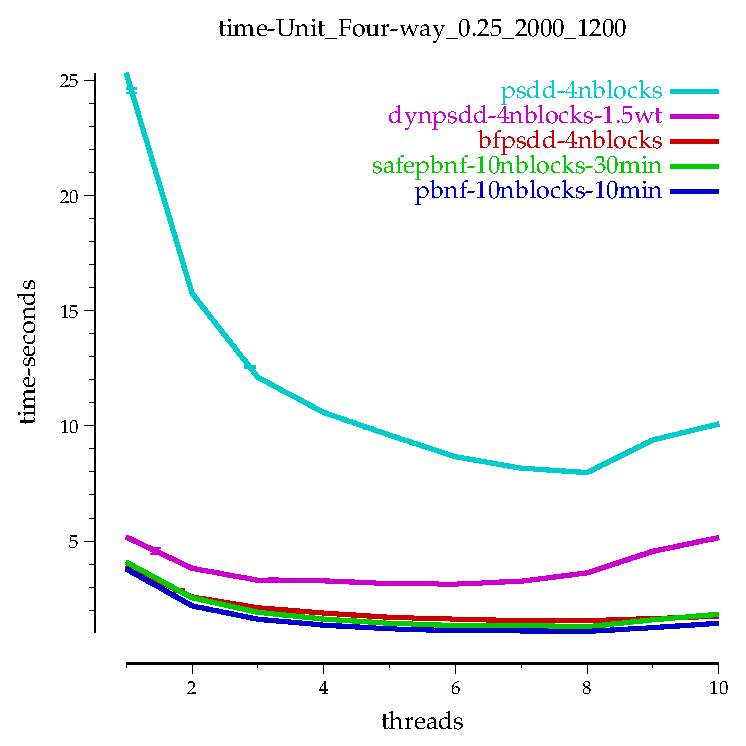
\includegraphics[width=4in,height=3in]{figures/time-Unit_Four-way_0_25_2000_1200}
  }
  \onslide*{3}{
    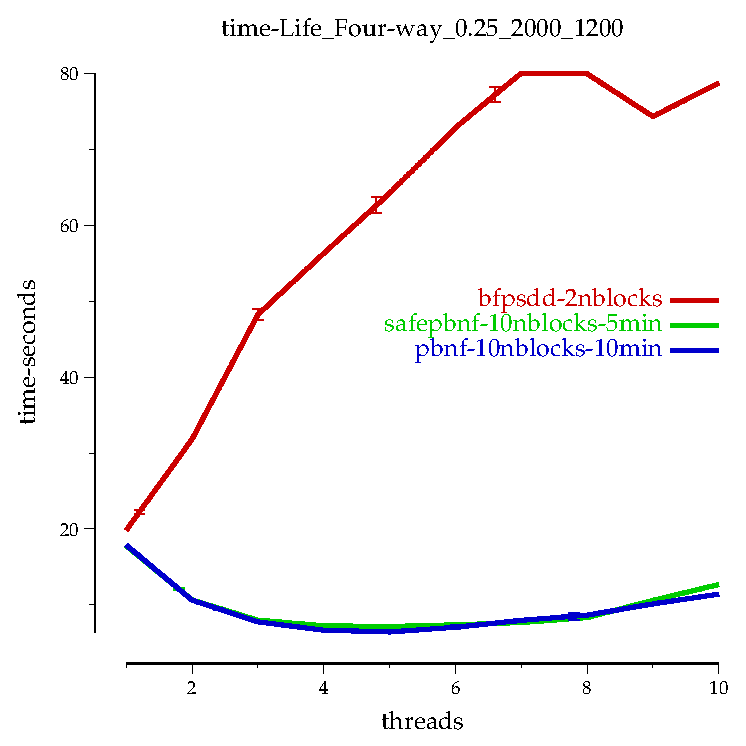
\includegraphics[width=4in,height=3in]{figures/time-Life_Four-way_0_25_2000_1200}
  }
\end{slide}

% --------------------

\begin{slide}{Sliding Tiles}
  \onslide*{1}{
    \begin{description}
    \item [Width] 7
    \item [Height] 2
    \item [Costs] Unit
    \item [Projection] The blank, and 1-tile.
    \end{description}
  }
  \onslide*{2}{
    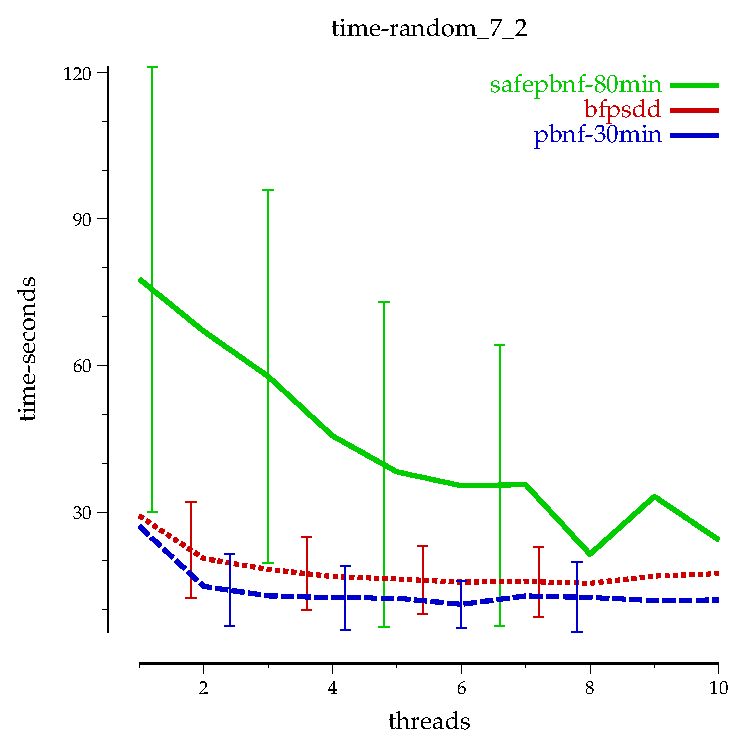
\includegraphics[width=4in,height=3in]{figures/time-random_7_2}
  }
\end{slide}

% ------------------------------------------------------------

\section{Conclusion}

% --------------------

\begin{slide}{Summary}
  \begin{center}
    Parallel Best NBlock First
  \end{center}
  \begin{itemize}
  \item Parallel best-first style search
  \item No synchronization in the ``fast-path''
  \item Performs well on a variety of domains \emph{without modification}
  \item Allows for \emph{many} possible variations:
    \begin{itemize}
    \item Weighted
    \item Pessimistic
    \item Optimistic
    \end{itemize}
  \item ``Hot Potato'' method prevents live-lock in infinite domains
  \end{itemize}
\end{slide}

% --------------------

\begin{slide}{Future Work}
  \begin{itemize}
  \item Test better grid world projections
  \item Test better tiles projections
  \item Evaluate the performance of iterative deepening PSDD
  \item Evaluate sub-optimal variants of PBNF
  \end{itemize}
\end{slide}

% --------------------

\begin{slide}{Questions}
\end{slide}{Questions}

% ------------------------------------------------------------

\end{document}
